\documentclass[landscape, two column, full page,reqno]{article}
\usepackage{mathrsfs}
\usepackage{amsmath,amssymb,amsthm,stmaryrd}
\usepackage[adobe-garamond]{mathdesign}
\AtBeginDocument{%
  \let\mathbb\relax
  \DeclareMathAlphabet\PazoBB{U}{fplmbb}{m}{n}%
  \newcommand{\mathbb}{\PazoBB}%
  \let\mathcal\relax
  \DeclareMathAlphabet{\OMScal}{OMS}{cmsy}{m}{n}
  \newcommand{\mathcal}{\OMScal}%
}
\usepackage{fontspec}
\usepackage{tikz}
\usetikzlibrary{arrows}
\usepackage{multicol}
\setmainfont[Numbers={Proportional,OldStyle}]{Adobe Garamond Pro}
%
%NATBIB
\usepackage[comma]{natbib}
%HYPERREF PACKAGE
\usepackage{xcolor}
\PassOptionsToPackage{hyphens}{url}
\usepackage[backref=page,linktocpage=true,colorlinks]{hyperref}
\renewcommand{\backrefxxx}[3]{[\hyperlink{page.#1}{#1}]}
\hypersetup{
    colorlinks = true,
    citecolor = blue,
    urlcolor = blue,
    filecolor = blue,
    linkcolor = blue,
}
%PATCH TO ONLY HYPERLINK YEAR OF CITATION
\usepackage{etoolbox}
\makeatletter
% Patch case where name and year are separated by aysep
\patchcmd{\NAT@citex}
  {\@citea\NAT@hyper@{%
     \NAT@nmfmt{\NAT@nm}%
     \hyper@natlinkbreak{\NAT@aysep\NAT@spacechar}{\@citeb\@extra@b@citeb}%
     \NAT@date}}
  {\@citea\NAT@nmfmt{\NAT@nm}%
   \NAT@aysep\NAT@spacechar\NAT@hyper@{\NAT@date}}{}{}
% Patch case where name and year are separated by opening bracket
\patchcmd{\NAT@citex}
  {\@citea\NAT@hyper@{%
     \NAT@nmfmt{\NAT@nm}%
     \hyper@natlinkbreak{\NAT@spacechar\NAT@@open\if*#1*\else#1\NAT@spacechar\fi}%
       {\@citeb\@extra@b@citeb}%
     \NAT@date}}
  {\@citea\NAT@nmfmt{\NAT@nm}%
   \NAT@spacechar\NAT@@open\if*#1*\else#1\NAT@spacechar\fi\NAT@hyper@{\NAT@date}}
  {}{}
\makeatother
%
%FOOTNOTE SPACING
\usepackage[hang,multiple,splitrule]{footmisc}
\setlength{\footnotemargin}{4mm}

%Titlesec package
\usepackage{titlesec}
%Centering and readjusting size of headings
\titleformat{\section}[hang]
{\normalfont\sc\filcenter}{\thesection}{1em}{}
\titleformat{\subsection}[hang]
{\normalfont\sc\filcenter}{\thesubsection}{1em}{}
\titleformat{\subsubsection}[hang]
{\normalfont\bf}{\thesubsubsection}{1em}{}
			% in the document preamble: 
				\let\endgraf\par % because LaTeX doesn't like \par 
			% in some command arguments 
				\let\subtitlefont\normalfont % or whatever 
				
\usepackage{enumitem}

\newcommand{\qd}{\begin{quote}\begin{description}  [align=left,style=nextline,leftmargin=*,labelsep=0pt,font=\normalfont]}
\newcommand{\zd}{\end{description}\end{quote}}
\newcommand{\qe}{\begin{enumerate}[align=left,style=nextline,leftmargin=17pt,labelsep=5pt,font=\normalfont]}
\newcommand{\qer}{\begin{enumerate}[align=left,style=nextline,leftmargin=17pt,labelsep=5pt,font=\normalfont , resume]}
\newcommand{\qei}{\begin{enumerate}[align=left,style=nextline,leftmargin=15pt, labelsep=10pt,font=\normalfont]}

\newcommand{\e}{\emph}
\newcommand{\fn}{\footnote}
\renewcommand{\P}{\mathcal{P}}
\newcommand{\tbf}{\textbf}
\newcommand{\ze}{\end{enumerate}}
\newcommand{\p}{\item}
\newcommand{\qq}[1]{ \ulcorner #1 \urcorner}
\newcommand{\thus}{

\vspace{5pt}
\hrule
}
\newcommand{\I}{\mathscr{T}}
\newcommand{\T}{[\mathscr{T}}
\newcommand{\V}[1]{\llbracket #1 \rrbracket}
\newcommand{\SV}[1]{S\hspace{-0.5pt}V_\mathscr{I}( #1 )}
\DeclareRobustCommand*{\modeled}{%
  \Relbar\joinrel\mathrel{|}
 %
}
\newcommand{\s}{\textsc}
\newcommand{\argu}[2]{\begin{center}\begin{minipage}{#1} \begin{enumerate}
	#2
\end{enumerate}
\end{minipage}  
\end{center}}

\title{Vagueness}
\author{M\&E Core}
\date{October 2nd, 2018}


\usepackage{layout}
\voffset = -40pt
\textheight = 450pt
\setlength{\columnsep}{20pt}
\begin{document}
%\layout
\twocolumn[{%
 \centering
\maketitle
}]



\section{The Sorites Paradox}
\qe
\p On the left, we have a collection of 1,000,000 grains of sand.  To its immediate right, there is a collection of 999,999 grains of sand.  To its immediate right, there is a collection of 999,998 grains of sand, and so on.  Finally, on the far right, we have a single grain of sand.  The sand on the far left is plainly a heap.  The single grain of sand on the far right is plainly not a heap.

\p Now, consider the following argument: %\fn{ `$H(x)$' means `a collection of $x$ grains of sand is a heap'.}
		\argu{150pt}{
		\p[] $H($1,000,000$)$
		\p[] $(\forall n ) (H(n) \to H(n-1))$
		\thus
		\p[] $H($1$)$
		}
Alternatively, consider \e{this} argument:
		\argu{160pt}{
		\p[] $\neg H($1$)$
		\p[] $(\forall n ) (\neg H(n) \to \neg H(n+1))$
		\thus
		\p[] $\neg H($1,000,000$)$
		}
		\qe
		\p The first premise of each of these arguments is plainly true.  Their second premises appear undeniable---how could adding or substracting a single grain of sand transform a heap into a non-heap, or a non-heap into a heap?  And the argument form appears to be valid.  But if we accept both of these arguments, then we have accepted an explicit contradiction.  So we have a paradox.  This paradox is known as the `sorites paradox', since the Greek word for `heap' is `sorites'.  We could easily run similar arguments with redness, baldness, thinness, coldness, or just about any predicate from English.
		\p Why not just reject the second premise of each argument?  Given classical logic, rejecting the second premise of these arguments commits you to 
				\[
				(\exists n) (H(n) \wedge \neg H(n-1))
				\]
		That is: it commits us to saying that there is a sharp cut off point for being a heap---that, for some $n$, while $n$ grains of sand is a heap, $n-1$ grains of sand is \e{not} a heap.  However, this appears false.  There is no number $n$ such that $n$ is a sharp cut off point for being a heap---one fewer, and you're not a heap.
		\ze 
\p The second premise of the sorites argument tells us that being a heap is a \e{tolerant} property---minor changes to the number of grains of sand do not make a difference with respect to whether something is a heap or not.   There are other properties which appear to be tolerant in the same way, and corresponding to each of them is a sorites argument.  For instance,
	\qe
	\p If a color is red, then, if you make an imperceptible change to the hue of the color, it will still be red.
	\p If a person is tall, then, if you make them 0.0000001 cm shorter, they will still be tall.
	\p If a person is rich, then, if you make them 1 cent poorer, they will still be rich.
	\p If a man is not bald, removing a single hair will not make him bald.
	\p[] $\vdots$
	\ze 
%\p We may worry about universal instantiation; but we may easily construct a version of the paradox which does not require it.
%		\argu{160pt}{
%		\p[] $H($1,000,000$)$
%		\p[] $H($1,000,000$) \to H($999,999$)$
%		\p[] $H($999,999$) \to H($999,998$)$
%		\p[] $\vdots$
%		\p[]  $H(n) \to H(n-1)$
%		\p[] $\vdots$
%		\p[]  $H($2$) \to H($1$)$
%		\thus
%		\p[] $H($1$)$
%		}



\section{Truth-Gap Theories}
\p A natural reaction to the sorites paradox is to think that, even though 1,000,000 grains of sand is clearly a heap, and 1 grain of sand is clearly \e{not} a heap, at some point in the middle, it stops being clear whether what you have is a  heap or not.  At some point in the middle, it is \e{vague} whether what we have is a heap or not.  (To use another common expression, at some point in the middle, we have \e{borderline} cases of heaps.)
	\qe
	\p When we say that it's not \e{clear} whether we have a heap or not---when we say that it is \e{vague} whether we have a heap or not---what does this mean?
	\p One possible answer: when it is vague whether we have a heap, it is neither absolutely true nor absolutely false that what we have is a heap.  Several theories of vagueness are built around this idea.\footnote{ On an approach we won't discuss, propositions have \e{degrees} of truth intermediate between $0$ and $1$.  On this treatment of vagueness, even though every premise of the sorites argument from point (3) is very nearly true, each application of \e{modus ponens} leaves us with a conclusion slightly less true, until eventually we end up with a conclusion which is completely false.  See Dorothy Edgington's ``{Vagueness by Degrees}'', in \emph{Vagueness: a Reader}, edited by Rosanna Keefe and Peter Smith.  MIT Press, Cambridge, MA.  Ch.~16 (pp.~294--316).}  Let's start with the simplest way of cashing this idea out: the recognition of a new truth-value: neither true nor false.
	\ze 
\subsection{ \L ukasiewicz's Trivalent Logic}			
\p \L ukasiewicz developed a logic which denies bivalence and accepts a third truth-value (`$\#$', which we can think of as `neither true nor false').   Before getting to this logic, a few points of clarification.
	\qe
	\p \e{Bivalence} is the claim that every proposition is either true or false.   
				\[
				T\langle \phi \rangle \vee F\langle \phi \rangle
				\]
(where, recall, $\qq{\langle \phi \rangle}$ denotes the proposition expressed by $\qq{\phi}$.) If we identify falsehood with the truth of a negation, $F\langle \phi \rangle \leftrightarrow T\langle \neg \phi \rangle$, then we may re-write bivalence as
				\[\tag{\s{Bivalence}}
				T\langle \phi \rangle \vee T\langle \neg \phi \rangle
				\]	
		\p This should be carefully distinguished from the law of excluded middle (\s{lem}).  \s{Lem} is the claim that $\phi \vee \neg \phi$ is a  tautology.
				\[\tag{\s{lem}}
				\models \phi \vee \neg \phi
				\]
		as we'll see, these two theses may come apart.
	\ze 
\p For \L ukasiewicz's logic, we're going to assume that we have an infinite collection of \e{atomic} sentence letters, 
	\[
	p, q, r, p_1, q_1, r_1, p_2, q_2, \dots
	\]				
which we may combine with the following logical connectives to form \e{compound} sentences in the usual way,
	\[
	\neg \,,\, \wedge \,,\, \vee \,,\, \to
	\]
\p In a \e{tri}valent logic, there are three possible truth-values, $1$, $0$, and $\#$, which we may understand as follows:
	\qe
	\p If $\qq{\phi}$ has the truth-value $1$, then $\qq{\phi}$ is true
	\p If $\qq{\phi}$ has the truth-value $0$, then $\qq{\phi}$ is false
	\p If $\qq{\phi}$ has the truth-value $\#$, then $\qq{\phi}$ is neither true nor false
	\ze 
\p A trivalent truth-value assignment, $\I$, assigns one of these three truth-values to every \underline{atomic} sentence.
		\qd
		\p[\s{Trivalent Truth-Value Assignment}] A trivalent truth-value assignment $\mathscr{T}$ is a function from atomic sentences to $\{ 1, 0, \# \}$.
				\qe
				\p If $\I(\alpha) = 1$, then $\qq{\alpha}$ is true on $\I$.
				\p If $\I(\alpha) = 0$, then $\qq{\alpha}$ is false on  $\I$.
				\p If $\I(\alpha) = \#$, then $\qq{\alpha}$ is neither true nor false on $\I$.
				\ze 
		\zd 
\p A trivalent truth-value assignment only tells us the truth-values of the \e{atomic} sentences.  In classical logic, the standard truth-tables tell us how to determine the truth-values of compound sentences from there.   In \L ukasiewicz's trivalent logic, we have the following truth-tables.
	\[
	\begin{array}{c | c}
	\neg	&	\\\hline
	1	&	0	\\
	0	&	1	\\
	\#	&	\#	
	\end{array}
	\quad
	\begin{array}{c | c c c}
	\wedge	&	1	&	0	&	\#	\\\hline
	1		&	1	&	0	&	\#	\\
	0		&	0	&	0	&	0	\\
	\#		&	\#	&	0	&	\#
	\end{array}
	\quad
	\begin{array}{c | c c c}
	\vee		&	1	&	0	&	\#	\\\hline
	1		&	1	&	1	&	1	\\
	0		&	1	&	0	&	\#	\\
	\#		&	1	&	\#	&	\#
	\end{array}
	\quad
	\begin{array}{c | c c c}
	\to		&	1	&	0	&	\#	\\\hline
	1		&	1	&	0	&	\#	\\
	0		&	1	&	1	&	1	\\
	\#		&	1	&	\#	&	1
	\end{array}
	\]
	\qe
	\p When reading these tables, the truth-value of the sentence to the left of the connective is given in the rows, and the truth-value of the sentence to the right of the connective is given in the columns.
	\p For instance, if $\qq{\phi}$ is true and $\qq{\psi}$ is neither true nor false, then these tables tell us that:
		\qe
		\p $\qq{\neg \psi}$ is neither true nor false,
		\p $\qq{\phi \wedge \psi}$ is neither true nor false,
		\p $\qq{\phi \vee \psi}$ is true, 
		\p $\qq{\phi \to \psi}$ is neither true nor false, and
		\p $\qq{\psi \to \phi}$ is true.
		\ze 
	\ze 
\p We should also say something about which \e{arguments} are valid.  Everything the logic has to say about validity is encapsulated in a \e{consequence} relation $\models_{\text{\L}}$, which is a binary relation between a \e{set} of sentences $\Gamma$ and a sentence $\phi$, written ${\Gamma \models_{\text{\L}} \phi}$.
		\qe
		\p In classical logic, we say that a set of sentences $\Gamma$ {entails} a sentence $\phi$ iff every \e{bivalent} truth-value assignment which makes all the sentences in $\Gamma$ true makes $\phi$ true also.
		\p Thus, there is a \e{designated} truth-value ($1$), and entailment is understood as the preservation of that designated truth-value.
		\p When we have three truth-values, we face a choice: we could say that the designated truth-value is \e{truth} ($1$), or we could say that the designated truth-value is \e{non-falsehood} (either $1$ or $\#$).  For \L ukasiewicz's logic, we say that $1$ is the designated truth-value.
		\p Thus, we say that $\Gamma \models_{\text{\L}} \phi$ iff every trivalent truth-value assignment which makes all the sentences in $\Gamma$ true makes $\qq{\phi}$ true  also.
		\ze 
	\subsubsection*{Exercises}
Use the \L uksiewicz truth-tables to determined whether the following claims are true:
	\qe
	\p $\{ p \to q \} \models_{\text{\L}} \neg p \vee q$
	\p $\{ \neg (p \vee q) \} \models_{\text{\e{\L}}} \neg p \wedge \neg q$
	\p $\models_{\text{\L}} p \to p$
	\ze 

\p What does this logic say about the sorites argument?  
	\qe
	\p It will say that one of its premises is not true (though no premise will be false).  
	\p For a simplistic case, suppose that we have only three cases: 1, 2, and 3.  And suppose that 3 is a clear case of the predicate $H$, 1 is a clear case of something which is not $H$, and 2 is a borderline case.   That is, we have the following trivalent truth-value assignment, $\I$,\footnote{ I'm carelessly flipping back and forth between propositional logic and predicate logic here.  Things get messier when we consider a trivalent predicate logic model---in rough outline, we have, for each predicate $F$, an \e{extension} and an \e{anti-extension}, and while we require that the extension and the anti-extension don't overlap, we allow that they don't cover the domain, so that some entities in the domain could fail to fall in either.  If `$a$' refers to such an entity, then `$F(a)$' is $\#$.}
			\[
			\begin{array}{ c | c}
			x		&		\I(H(x))		\\\hline
			\text{3}	&		1			\\
			\text{2}	&		\#			\\
			\text{1}	&		0
			\end{array}	
			\]
	\p Then, the sorites argument would be:
			\argu{100pt}{
			\p[] $H($3$)$
			\p[] $H($3$) \to H($2$)$
			\p[] $H($2$) \to H($1$)$ 
			\thus
			\p[] $H($1$)$
			}
	And, while the 1st premise is true, the 2nd and 3rd premises are neither true nor false.  So the argument is invalid, according to the \L ukasiewicz logic.
	\p In classical logic, saying that the 2nd premise is not true means saying that it is false, which means saying that its negation is true, which means saying that 
		\[
		H(\text{3}) \wedge \neg H(\text{2})
		\] 
	which is to say: removing a single grain of sand can turn a heap into a non-heap.  Notice that, in a trivalent logic, we no longer have to say this.  For we can deny that the 2nd premise is true without affirming that it is false, or that its negation is true.  In fact, if the 2nd premise is neither true nor false, then its negation will also be neither true nor false.  So, in a trivalent logic, we do not have to affirm that removing a single grain of sand can transform a heap into a non-heap.  
	\ze 
 \subsection{Higher-Order Vagueness}
 \p Notice, however, that on this logic, removing a single grain of sand \e{can} transform a clear heap into a borderline heap.
% \subsection{\L ukasiewicz's Trivalent Logic with Determinacy}
	\qe
	\p Suppose we introduce the operator `$\Delta$' for \e{Determinacy}.  That is, $\qq{\Delta \phi}$ means $\qq{\text{It is determinately the case that } \phi }$.   We could give $\Delta$ the following truth-table.
		\[
		\begin{array}{c | c}
		\Delta	&	\\\hline
		1	&	1	\\
		0	&	0	\\
		\#	&	0	
		\end{array}
		\]
	Note: given this operator for `it is determinate that', we may define a corresponding operator for `it is indeterminate whether': \[\nabla \phi \stackrel{\text{\tiny def}}{=} \neg \Delta \phi \wedge \neg \Delta \neg \phi\]
	\p Then, in our simple case from above, we would accept that there is a sharp cut-off point between being a \e{determinate} heap and not being a determinate heap.
		\[
		\Delta H(\text{3}) \wedge \neg \Delta H(\text{2})
		\]
	\ze 
\p However, it appears that we can construct a sorites argument with the property of being a \e{determinate} heap.
	\argu{150pt}{
	\p[] $\Delta H ($1,000,000$)$
	\p[] $(\forall n) (\Delta H(n) \to \Delta H(n-1))$
	\thus
	\p[] $\Delta H($1$)$
	}
	\qe
	\p Being a determinate heap \e{also} appears to be a tolerant property.  If you have a determinate heap, then, if you remove a single grain of sand, what you get will also be a determinate heap.
	\p This is the problem of \e{higher-order vagueness}.  There is not only \e{first-order vagueness}, in the sense that there is some sand which is neither clearly a heap nor clearly not a heap.  There is additionally \e{second-order vagueness}, in the sense that there is some sand which is neither clearly \e{clearly} a heap nor clearly \e{not}  clearly a heap.
		\qe
		\p So too does there appear to be \e{third}-order vagueness, and \e{fourth}-order vagueness, and so on and so forth.
		\ze 
	\p The logic of \L ukasiewicz  does not appear to be able to accommodate the phenomenon  of higher-order vagueness; for that logic says it is a tautology that, if it is determinate that $\phi$, then it is determinate that it is determinate that $\phi$:
				\[
				\models_{\text{\L}} \Delta \phi \to \Delta \Delta \phi
				\]
	\ze 

\subsection{Penumbral Connections}
\p Another problem for the \L ukasiewicz logic:  Suppose that `$p$' is neither true nor false.  Then, by \L ukasiewicz table for $\neg$, `$\neg p$' is neither true nor false.  Then,
	\qe
	\p By the by \L ukasiewicz table for $\vee$, `$p \vee \neg p$' is neither true nor false.  So \s{lem} is not a tautology.
							\[
							\not\models_{\text{\L}} p \vee \neg p
							\]
	\p By the by \L ukasiewicz table for $\wedge$, `$p \wedge \neg p$' is neither true nor false.  So, by the table for $\neg$, `$\neg(p \wedge \neg p)$' is neither true nor false.  So the law of noncontradiction is not a tautology, either.
							\[
							\not\models_{\text{\L}} \neg (p \wedge \neg p)
							\]
	\ze 
\p Even when matters are indeterminate, there appear to be important connections between those  indeterminate matters.  For instance,
	\qe
	\p Either I'm bald or I'm not bald.
	\p If 55$^\circ$ is cold, then 50$^\circ$ is cold, too.
	\p John isn't both rich and not rich.
	\ze 
These connections between indeterminate propositions are known as \e{penumbral connections}.


\subsection{Supervaluationism}
\p Supervaluationism attempts to accomodate these kinds of penumbral connections.
	\qe
	\p A standard way of understanding supervaluationism is like this: vagueness is a linguistic affair.  What accounts for the vagueness of expressions like `red', `heap', `rich', `bald', and so on is that we haven't made our minds up about how exactly to use those terms.  We've decided that we should use the word `heap' to describe 1,000,000 grains of sand, and we've decided that we shouldn't use it to describe  1 grain of sand, but we've not really made up our minds about when something goes from a heap to a non-heap.
	\p Nevertheless, we \e{have} made up our minds that, \e{if} $n$ grains of sand is a heap, then $n+1$ is, too.  Likewise, we've made up our mind that any sand either is or is not a heap.  And we've made up our mind that no sand is \e{both} a heap \e{and} not a heap.
	\ze 
\p More formally, the idea behind supervaluationism is this: when we use our terms, we haven't gotten \e{precise} about what they mean.  So it's not currently settled what those terms mean.  However, there are a bunch of acceptable ways of taking our current usage and \e{precisifying} it.  And a sentence is true if it comes out true given \e{every} admissible precisification of our language.
	\qd
	\p[\s{Supervaluationism}]  A sentence is true iff it is true on every admissible precisification of our language.  A sentence is false iff it is false on every admissible precisification of our language.  Otherwise, the sentence is neither true nor false.  
	\zd 
\p We can develop this into a formal logic for our simple propositional language as follows:
	\qe
	\p Given a trivalent truth-value assignment $\I$, we may define the notion of a \e{precisification}, $\P$, of that trivalent truth-value assignment:
	\qd	\p[\s{Precisification}] $\P$ is a bivalent \e{precisification} of a trivalent truth-value assignment $\I$ iff, for all atomic sentences $\qq{\alpha}$,
		\qe
		\p Either $\P(\alpha) = 1$ or $\P(\alpha) = 0$
		\p If $\I({\alpha}) = 1$, then $\P({\alpha }) = 1$
		\p If $\I({\alpha}) = 0$, then  $\P({\alpha}) = 0$
		\ze
	\zd
	\p That is, the precisification of a trivalent truth-value assignment agrees with that trivalent truth-value assignment about the classical truth-values $1$ and $0$, but settles the indeterminacy one way or the other.
	\ze 
\p Supervaluationism then says that a sentence $\qq{\phi}$ is true on the trivalent truth-value assignment $\I$ iff $\qq{\phi}$ is true on every precisification $\P$ of $\I$.  Similarly, a sentence $\qq{\phi}$ is false on $\I$ iff $\qq{\phi}$ is false on every precisification $\P$ of $\I$.  Finally, if $\qq{\phi}$ is true on some precisifications of $\I$ and false on others, then $\qq{\phi}$ is neither true nor false on $\I$.
		\qe
		\p Now, consider a truth-value assignment $\I$ on which `$p$' is neither true nor false, $\I(p) = \#$.  One precisification of $\I$ is $\I_1$, according to which `$p$' is true; the other is $\I_0$, according to which $p$ is false.  On both these precisifications, `$p \vee \neg p$' is true.  So the supervaluationist says that `$p \vee \neg p$' is true on the trivalent truth-value assignment $\I$.
		\p Similarly, on both $\I_1$ and $\I_0$, `$p \wedge \neg p$' is false.  So the supervaluationist says that `$p \wedge \neg p$' is false on the trivalent truth-value assignment $\I$.
		\ze 
\p When it comes to the question of which arguments are valid and which are invalid, the supervaluationist faces choices.
	\qe
	\p In the first place, there is the choice of which truth-value to take as the designated truth-value.  We will assume that the supervaluationist says it is \e{truth}, and not \e{non-falsehood}. 
	\p Then, the most natural thing for the supervaluationist to say is that a valid argument is one that preserves \e{truth}---that is, the argument from the sentences in $\Gamma$ to $\qq{\phi}$ is super-valuationistically valid,
			\[
			\Gamma \models_{SV} \phi
			\]
	iff every trivalent truth-value assignment which makes all the sentences in $\Gamma$ true makes $\phi$ true as well.
	\p However, they could attempt to super-valuate with respect to validity as well.  That is, they could attempt to say that $\Gamma$ entails $\qq{\phi}$,	
			\[
			\Gamma \models^*_{SV} \phi
			\]
		iff, for every trivalent truth-value assignment $\I$, every precisification of $\I$ which makes all of the sentences in $\Gamma$ true makes $\qq{\phi}$ true as well.
		\p The first of these approaches is called \e{global} validity, whereas the second is called \e{local} validity.  We will assume that the supervaluationist opts for global validity in what follows.
	\ze 
\p Notice, then, that even though the supervaluationist denies bivalence, they still accept the law of the excluded middle, \s{lem}.  
	\qe
	\p Take a borderline sentence `$p$'.  There will be some precisifications on which `$p$' is true, and some on which it is false.  On the precisifications which make `$p$' true, `$p \vee \neg p$' will be true.  On the precisifications which make `$p$' false, `$\neg p$' will be true, so that `$p \vee \neg p$' will be true.  So `$p \vee \neg p$' will be true even when `$p$' is neither true nor false.
	\p In general, prenumbral connections between sentences of the language will be preserved on a supervaluationistic approach.  On any precisification of `cold', if 55$^\circ$ is cold, then 50$^\circ$ will be cold, also.  So it will be true that, if 55$^\circ$ is cold, then 50$^\circ$ is cold as well.    However, there are some precisifications of `cold' on which `if 50$^\circ$ is cold, then 55$^\circ$ is cold' is false.  So it will not be true that, if 50$^\circ$ is cold, then 55$^\circ$ is cold, too.
	\ze 
\p In general, the supervaluationist's logic is just classical logic.  That is to say, an argument is valid according to the supervaluationist iff that argument is valid according to classical logic.
	\qe
	\p That is, if we use `$\models$' for the classical logician's consequence relation, then 
			\[
			\Gamma \models \phi \quad\iff\quad \Gamma \models_{SV} \phi
			\]
	\ze 
\p What does the supervaluationist say about the sorites?
	\qe
	\p They will say that the second premise of the argument,
				\[
				(\forall n)(H(n) \to H(n-1))
				\]
		is false (not only not true, but \e{false}).  For this premise is false on every precisification of the extension of $H$.  Moreover, because they preserve classical logic, they will assert the negation of the second premise,
				\[
				(\exists n)(H(n) \wedge \neg H(n-1))
				\]
		That is, they will say that there is a sharp cut-off point between being a heap and being a non-heap.
	\p However, there is no number $n$ for which they will say that `$H(n) \wedge \neg H(n+1))$' is true.  That is, they will say that an existential generalization `$(\exists x) \phi x$' is true, even though there is nothing `$x$' could refer to such that `$\phi x $' is true.  This is for essentially the same reason that they will endorse `$p \vee q$' without endorsing either `$p$' or `$q$'.
	\ze 
\subsection{Supervaluationism with Determinacy}

\p We may introduce an additional operator `$\Delta$', for \e{Determinacy}.  In order to explain the logic of the determinacy operator, we should be a bit more explicit and careful about how we are determining the truth-value of logically complex sentences from a given truth-value assignment.  To keep things simple, let's begin with the classical case.
	\qe
	\p Given a {classical}, \e{bivalent} truth-value assignment $\P$, which is just a function from \e{atomic} sentences to $\{ 1, 0 \}$, we may construct the \e{valuation} function, $\V{~}^\P$, which is a function from \e{any} sentence to $\{ 1, 0 \}$.  In order to count as a valuation function for the truth-value assignment $\P$, $V{~}^\P$ must satisfy the following conditions, for any atomic sentence $\qq{\alpha}$ and any sentences $\qq{\phi}$ and $\qq{\psi}$:
		\qe
		\p[$\alpha$)] $\V{\alpha}^\P = \P(\alpha)$.
		\p[$\neg$)] $\V{\neg \phi}^\P = 1$ iff $\V{\phi}^\P = 0$.
		\p[$\vee$)] $\V{\phi \vee \psi}^\P = 1$ iff $\V{ \phi}^\P = 1$ or $\V{\psi}^\P = 1$.
		\p[$\wedge$)] $\V{\phi \wedge \psi}^\P = 1$ iff $\V{\phi}^\P = 1$ and $\V{\psi}^\P = 1$.
		\p[$\to$)] $\V{\phi \to \psi}^\P = 1$ iff $\V{ \phi}^\P = 0$ or $\V{\psi}^\P = 1$.
		\ze 
%	\p Similarly, given a \e{trivalent} truth-value assignment $\I$, we may construct a trivalent {valuation} function $\V{~}^\I$.  This is a function from \e{any} sentence to $\{ 1, 0, \# \}$.  In order to count as a valuation function for the truth-value assignment $\I$, $\V{~}^\I$ must satisfy the following conditions, for any atomic sentence $\qq{\alpha}$ and any sentences $\qq{\phi}$ and $\qq{\psi}$:
%		\qe
%		\p[$\alpha$)] $\V{\alpha}^\I = \I(\alpha)$.
%		\p[$\neg$)] $\V{\neg \phi}^\I = 1$ iff $\V{\phi}^\I = 0$, and $\V{\neg \phi}^\I = \#$ iff $\V{\phi}^\I = \#$. 
%		\p[$\vee$)] $\V{\phi \vee \psi}^\I = 1$ iff $\V{ \phi}^\I = 1$ or $\V{\psi}^\I = 1$, $\V{\phi \vee \psi}^\I = 0$ iff both $\V{\phi}^\I = 0$ and $\V{\psi}^\I = 0$, and $\V{\phi \vee \psi}^\I = \#$ otherwise.
	%	\p[$\wedge$)] $\V{\phi \wedge \psi}^\I = 1$ iff both $\V{\phi}^\P = 1$ and $\V{\psi}^\P = 1$.  $\V{\phi \wedge \psi}^\I = 0$ if either $\V{\phi}^\I = 0$ or $\V{\psi}^\I = 0$.  And $\V{\phi \wedge \psi}^\I = \#$ otherwise.
%		\p[$\to$)] $\V{\phi \to \psi}^\I = 1$ iff $\V{ \phi}^\I = 0$,  $\V{\psi}^\P = 1$, or $\V{\phi}^\I = \V{\psi}^\I = \#$.
%		\ze 
%	(These clauses simply encode the \L ukasiewicz tables from above.)
	\p Now, given a trivalent truth-value assignment $\I$, we may construct a \e{super}valuation function, $\V{~}^\I$.  In order to count as a supervaluation for truth-value assignment $\I$, $\V{~}^\I$ must satisfy the following conditions, for any sentence $\qq{\phi}$:
		\qe
		\p[0)] If, for every precisification $\P$ of $\I$, $\V{\phi}^\P = 1$, then $\V{\phi}^\I = 1$.
		\p[1)] If, for every precisification $\P$ of $\I$, $\V{\phi}^\P = 0$, then $\V{\phi}^\I = 0$.
		\p[\#)] If, for some precisification $\P$ of $\I$,  $\V{\phi}^\P = 1$, and, for some precisification $\P$ of $\I$, $\V{\phi}^\P = 0$, then $\V{\phi}^\I = \#$.
		\ze 
	\p Notice that we may think of each precisification $\P$ of $\I$ as a \e{possible world}.  Supervaluationist truth is then tantamount to necessary truth (truth at all precisifications).  Supervaluationist falsehood is tantamount to necessary falsehood (falsehood at all precisifications).  And the supervaluationist's indeterminacy is tantamount to contingency (truth at some precisifications, falsehood at others). 
	\ze  
\p Now, we may introduce the determinacy operator $\Delta$.    The trick is to think about it as a necessity modal like $\Box$.
	\qe
	\p Suppose we are given a trivalent truth-value assignment $\I$.  Then, we may consider all the precisifications $\P$ of $\I$ (think of each of these as a possible world).
	\p On any particular one of those precisifications, in order for a function $\V{~}^\P$, from sentences to $\{ 0, 1 \}$, to count as a  valuation function, it  must satisfy the rules ($\alpha$), ($\neg$), ($\vee$), ($\wedge$), and ($\to$), as above, and it must also satisfy the rule ($\Delta$), for any sentence $\phi$:
		\qe
		\p[$\Delta$)] $\V{\Delta \phi}^\P =1$ iff, for every precisification $\P^*$ of $\I$, $\V{\phi}^{\P^*} = 1$.
		\ze 
	(Once again, we may define an operator for `it is indeterminate whether', $\nabla \phi \stackrel{\text{\tiny def}}{=} \neg \Delta \phi \wedge \neg \Delta \neg \phi$.)
	\p And, once again, in order for a function $\V{~}^\I$, from sentences to $\{ 1, 0, \# \}$, to count as a \e{super}valuation for the interpretation $\I$, $\V{~}^\I$ must satisfy the following conditions, for any sentence $\qq{\phi}$:
		\qe
		\p[0)] If, for every precisification $\P$ of $\I$, $\V{\phi}^\P = 1$, then $\V{\phi}^\I = 1$.
		\p[1)] If, for every precisification $\P$ of $\I$, $\V{\phi}^\P = 0$, then $\V{\phi}^\I = 0$.
		\p[\#)] If, for some precisification $\P$ of $\I$,  $\V{\phi}^\P = 1$, and, for some precisification $\P$ of $\I$, $\V{\phi}^\P = 0$, then $\V{\phi}^\I = \#$.
		\ze 
	\ze 

	
\p Is it true that $p \models_{SV} \Delta p$?
	\qe
	\p Pick any trivalent truth-value assignment $\I$.  If $p$ is to be true on $\I$, then $p$ must be true on all of $\I$'s  precisifications.  So $\Delta p$ must be true on all of $\I$'s precisifications.  So $\Delta p$ must be true on $\I$.  So any trivalent truth-value assignment which makes the premise true must make the conclusion true as well, and the argument is valid.
	\ze 
\p What about the argument $\neg \Delta p \models_{SV} \neg p$?
	\qe
	\p Consider a trivalent truth-value assignment $\I$ according to which $p$ is neither true nor false.  Then, for every precisification $\P$ of $\I$, $\Delta p$ will be false.  Thus, for every precisification $\P$ of $\I$, `$\neg \Delta p$' will be true.  So `$\neg \Delta p$' is true on $\I$.  However, for some precisification $\P$ of $\I$, `$p$' will be true, so that `$\neg p$' will be false.  So `$\neg p$' will be neither true nor false.  So not every interpretation which makes the premise `$\neg \Delta p$' true will also make the conclusion `$\neg p$' true.  So the argument is invalid.
	\ze 
\p Now, again, we may say that an argument is valid according to the supervaluationist iff every trivalent truth-value assignment which makes all of its premises true makes its conclusion true also.
	\qe
	\p That is, we once again opt for \e{global} validity.
	\ze 
\p  Consider the sentence `$p \to \Delta p$'.  Is this sentence valid (is it a tautology)?
	\qe
	\p Consider a trivalent truth-value assignment $\I$ according to which $\I(p) = \#$.  Then, there is a precisification of $\I$, $\P_1$, on which $p$ is true, and there is a precisification of $\I$, $\P_0$, on which $p$ is false.   So, on every precisification, $\Delta p$ is false.   On $\I_0$, `$p \to \Delta p$' is true because `$p$' is false.  But, on $\I_1$, `$p \to \Delta p$' is false, since `$p$' is true but `$\Delta p$' is false.  So `$p \to \Delta p$' is true on some precisifications of $\I$ and false on others.  So `$p \to \Delta p$' is neither true nor false on the interpretation $\I$.
	\ze 
\p What this shows us is that contraposition (if $\phi \models \psi$, then $\neg \psi \models \neg \phi$) and conditional proof (if $\phi \models \psi$, then $\models \phi \to \psi$) are invalid for the supervaluationist, once we include the determinacy operator $\Delta$ in our language.

%\p Suppose that we want the $T$-schema to be valid (bracket worries about the liar paradox for the moment)
%		\[\tag{T}\label{T}
%		\models_{S} T(\qq{\phi}) \leftrightarrow \phi
%		\]
%	and suppose also that we accept the following consequence of supervaluationism with determinacy:
%		\[\tag{$\Delta$}\label{det}
%		\models_S \phi \leftrightarrow \Delta \phi
%		\]
%	\qe
%	\p Then, replacing the left-hand-side of \eqref{det} with the right-hand-side of \eqref{T}, we get
%			\[
%			\models_S T(\qq{\phi}) \leftrightarrow \Delta \phi
%			\]
%	\p And then, replacing the $\qq{\phi}$ on the right-hand-side with the left-hand-side of \eqref{T}, we get
%			\[
%			\models_S T(\qq{\phi}) \leftrightarrow \Delta T(\qq{\phi})
%			\]
%		which tells us, in the object language, that for Supervaluationism, truth just is determinate truth.
%	\ze 

\p How does the supervaluationist accommodate higher-order vagueness?
	\qe
	\p Keefe says that we should recognize higher-order vagueness as stemming from vagueness in the meta-language.  According to the supervaluationist, when they are speaking in the meta-language, there are a range of acceptable, or \e{admissible}, {precisifications} of our language.  However, the term `admissible precisification' is itself vague.  So it's not determinate whether \e{this} or \e{that} counts as an admissible precisification of our language, and so it's not determinate what the cut off is between the determinate and the borderline.
	\p The maneuver could be iterated with respect to the \e{meta-meta}-language, and with respect to the \e{meta-meta-meta}-language, and so on and so forth.
	\ze 
\begin{figure}[h!]
\centering
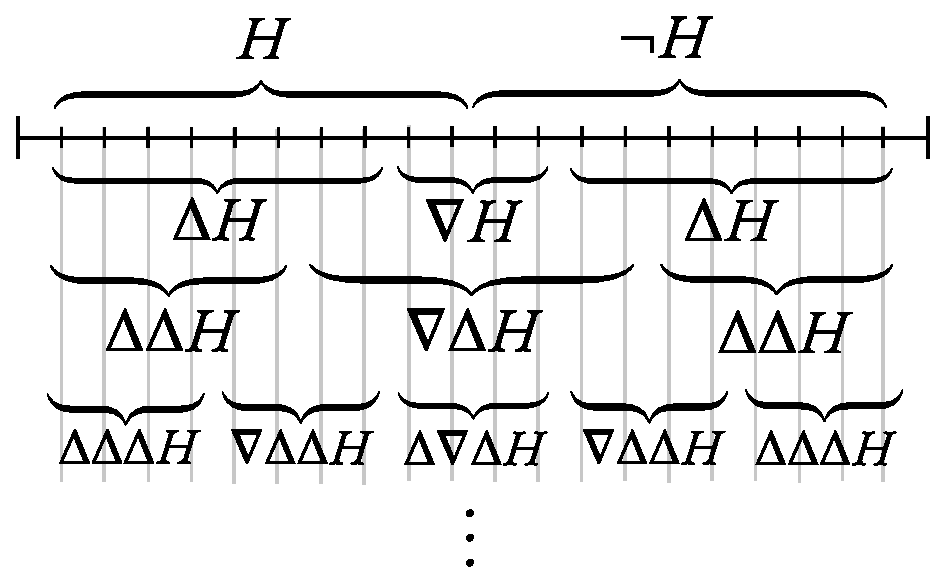
\includegraphics[scale=0.5]{hovagueness.eps}
\caption{Higher-Order Vagueness}
\end{figure}
\ze 

\end{document}
